\documentclass[fontsize=12pt, paper=a4, headinclude, twoside=false, 
parskip=half+,
pagesize=auto, numbers=noenddot, open=right, toc=listof, toc=bibliography]{scrreprt}

\usepackage{etex}% bei vielen packages


% PDF-Kompression
\pdfminorversion=5
\pdfobjcompresslevel=1

% CSV
%\usepackage{pgfplotstable}

% Allgemeines
\usepackage[automark]{scrpage2} % Kopf- und Fußzeilen
\usepackage{amsmath,marvosym} % Mathesachen
\usepackage[T1]{fontenc} % Ligaturen, richtige Umlaute im PDF
\usepackage[utf8]{inputenc}% UTF8-Kodierung für Umlaute usw
%\usepackage[ansinew]{inputenc}%windows
\usepackage{blindtext}


% Schriften
\usepackage{mathpazo} % Palatino für Mathemodus
%\usepackage{mathpazo,tgpagella} % auch sehr schöne Schriften
\usepackage{setspace} % Zeilenabstand
\onehalfspacing % 1,5 Zeilen


% Schriften-Größen
\setkomafont{chapter}{\Huge\rmfamily} % Überschrift der Ebene
\setkomafont{section}{\Large\rmfamily}
\setkomafont{subsection}{\large\rmfamily}
\setkomafont{subsubsection}{\large\rmfamily}
\setkomafont{chapterentry}{\large\rmfamily} % Überschrift der Ebene in Inhaltsverzeichnis
\setkomafont{descriptionlabel}{\bfseries\rmfamily} % für description Umgebungen




%\usepackage{dirtree}
% Sprache: Deutsch
\usepackage[ngerman]{babel} % Silbentrennung


% PDF
 \usepackage[ngerman,  pdfauthor={David Drost, Edward Kupfer, Hendrik Sawade, Tobias Wenzel}, pdftitle={Digital Text Forensics Search}, breaklinks=true]{hyperref}


\usepackage[final,stretch=40]{microtype} % mikrotypographische Optimierungen
\usepackage{url} % ermögliche Links (URLs)
\usepackage{pdflscape} % einzelne Seiten drehen können


% Tabellen

\usepackage{tabularx} % Für Tabellen mit vorgegeben Größen
\usepackage{longtable} % Tabellen über mehrere Seiten
\usepackage{array}%% 


%%  Bibliographie


\usepackage[round,authoryear]{natbib}
\bibliographystyle{mlu_ifg}
%\usepackage{bibgerm} % Umlaute in BibTeX
%\addbibresource{bibliography.bib}


\usepackage{float}

% Bilder
\usepackage{graphicx} % Bilder
\usepackage{color} % Farben
\graphicspath{{./img/}}
\DeclareGraphicsExtensions{.pdf,.png,.jpg} % bevorzuge pdf-Dateien
\usepackage{subfig}% http://ctan.org/pkg/subfig % Das scheint das neue zu sein.

\usepackage{caption}

\captionsetup{font=small,labelfont=bf,format=plain,labelsep=colon,justification=justified}
\captionsetup[subtable]{position=top}



% Quellcode
\usepackage{listings} % für Formatierung in Quelltexten
\definecolor{grau}{gray}{0.25}
\lstset{
	extendedchars=true,
	basicstyle=\tiny\ttfamily,
	%basicstyle=\footnotesize\ttfamily,
	tabsize=2,
	keywordstyle=\textbf,
	commentstyle=\color{grau},
	stringstyle=\textit,
	numbers=left,
	numberstyle=\tiny,
	% für schönen Zeilenumbruch
	breakautoindent  = true,
	breakindent      = 2em,
	breaklines       = true,
	postbreak        = ,
        showstringspaces=false,
	prebreak         = \raisebox{-.8ex}[0ex][0ex]{\Righttorque},
}
% Pseudocode
\usepackage{algorithm}
\usepackage[]{algpseudocode}
% linksbündige Fußboten
\deffootnote{1.5em}{1em}{\makebox[1.5em][l]{\thefootnotemark}}

\typearea{14} % typearea berechnet einen sinnvollen Satzspiegel (das heißt die Seitenränder) siehe auch http://www.ctan.org/pkg/typearea. Diese Berechnung befindet sich am Schluss, damit die Einstellungen oben berücksichtigt werden

\usepackage{scrhack} % Vermeidung einer Warnung


% Eigene Befehle %%%%%%%%%%%%%%%%%%%%%%%%%%%%%%%%%%%%%%%%%%%%%%%%%5



\usepackage{import} %zum importieren von Grafiken mit dem richtigen Pfad
\usepackage[%
%disable,  % uncomment this line to hide the comments!
textsize=footnotesize
]{todonotes}
\usepackage{xspace}
\newcommand{\comment}[1]{\todo[color=blue!40]{#1}\xspace{}}
\usepackage{soul}


% Abkürzungsverzeichnis
\usepackage{acronym}


% Sonstiges
\usepackage{booktabs}
\usepackage{arydshln}
\usepackage{eurosym}

\newcommand{\rowgroup}[1]{\hspace{-1em}#1}



\newlength{\spaltenbreite}
\spaltenbreite6cm
\usepackage{array}
\usepackage{booktabs,colortbl}
\definecolor{Gray}{gray}{0.9}
\usepackage{siunitx} % Formats the units and values
\usepackage{rotating}
\usepackage{physics}
\DeclareMathOperator*{\argmin}{arg\,min}
\DeclareMathOperator*{\argmax}{arg\,max}


\lstdefinestyle{mystyle}{
  basicstyle=%
    \ttfamily
    \lst@ifdisplaystyle\normalsize\fi
}
\lstset{style=mystyle}


% Weitere spezifische Pakete und Befehle
\usepackage{pgfplots}
\newcommand\gauss[2]{1/(#2*sqrt(2*pi))*exp(-((x-#1)^2)/(2*#2^2))} 
%penalty100 macht, dass Matlab in der nächsten Zeile landet.

% Showframe zeigt dir den Rand an. Dann kannt du sehen, ob irgendwas übersteht
%\usepackage{showframe}
%% Beispiele für korrekte Kodierungen.

\newcommand{\matlab}{MATLAB\textsuperscript{\textregistered}\xspace}
\newcommand{\coder}{\penalty100 MATLAB Coder\textsuperscript{\texttrademark}\xspace}
\newcommand{\prtools}{\penalty100 PRTools\xspace}
\newcommand{\fann}{\penalty100 FANN\xspace}

\newcommand{\pdfbox}{Apache PDFBox\textsuperscript{\textregistered}\xspace}

\newcommand{\tika}{\penalty100 Apache Tika\textsuperscript{\texttrademark}\xspace}


%ceil 
\usepackage{mathtools}
\DeclarePairedDelimiter{\ceil}{\lceil}{\rceil}

% UML
% \usepackage{tikz}
% \usepackage{../../tikz-uml}
% \usepackage{ifthen}
% \usepackage{xstring}
% \usepackage{calc}
% \usepackage{pgfopts}
% \tikzumlset{font=\tiny}


\usepackage{bytefield}
\setlength{\parfillskip}{0.5em plus 1fil} % don't fill the last line
\setlength{\emergencystretch}{.1\textwidth} % not to get preposterously bad lines

%%% Local Variables:
%%% mode: latex
%%% TeX-master: "arbeit"
%%% End:
 % Importiere die Einstellungen aus der 




% hier beginnt der eigentliche Inhalt
\begin{document}
\pagenumbering{Roman} % Seitenummerierung mit großen römischen Zahlen 
\pagestyle{empty} % kein Kopf- oder Fußzeilen auf den ersten Seiten

% Titelseite
\clearscrheadings\clearscrplain
\begin{center}

  
\includegraphics[width=.4\textwidth]{./img/uni_leipzig_logo}\\

  
  \begin{Large}
    \textbf{Digital Text Forensics Search}\\
  \end{Large}
  \vspace{8 mm}
 Information Retrieval\\ WS 2017/2018\\
  

	\vfill
	\normalsize
	\newcolumntype{x}[1]{>{\raggedleft\arraybackslash\hspace{0pt}}p{#1}}
	\begin{tabular}{x{6cm}p{7.5cm}}
		\rule{0mm}{5ex}\textbf{Betreuer:} & Martin Potthast
		\newline martin.potthast@uni-leipzig.de\\
          
		\rule{0mm}{5ex}\textbf{Autor:} & David Drost
		\newline dd42cequ@studserv.uni-leipzig.de
		\newline Matrikelnummer: 3724248\\ 
		
		\rule{0mm}{5ex}\textbf{Autor:} & Edward Kupfer
		\newline ek96foje@studserv.uni-leipzig.de
		\newline Matrikelnummer: 3709296\\ 

		\rule{0mm}{5ex}\textbf{Autor:} & Hendrik Sawade  
		\newline hs34byhe@studserv.uni-leipzig.de 
		\newline Matrikelnummer: 3745956 \\ 
                
		\rule{0mm}{5ex}\textbf{Autor:} & Tobias Wenzel 
		\newline tw54byka@studserv.uni-leipzig.de 
		\newline Matrikelnummer: 3733301 \\ 
	
		
		\rule{0mm}{5ex}\textbf{Abgabedatum:} & Leipzig, den \today \\ 
	\end{tabular} 

\end{center}
\clearpage

%%% Local Variables:
%%% mode: latex
%%% TeX-master: "arbeit"
%%% End:


\pagestyle{useheadings} % normale Kopf- und Fußzeilen für den Rest
\setcounter{tocdepth}{3}    % 3 = schließe auch subsubsections ein
\setcounter{secnumdepth}{3} % 3 = verleihe auch Bezifferung für subsubsections

\tableofcontents % erstelle hier das Inhaltsverzeichnis



%%% könnt ihr gerne benutzen, seh hier aber keinen Mehrwert.

%% \addchap{Abkürzungsverzeichnis}
%% \begin{acronym}
%%   %%\acro{NN}{Neural Network, dt. Neuronales Netzwerk}
%% \end{acronym}



\pagenumbering{arabic} % ab jetzt die normale arabische Nummerierung


\chapter{Einleitung}\label{ch:intro}
Ziel des Praktikums war es, eine themenspezifische Suchmaschine zu
implementieren, die wissenschaftliche Publikationen aus dem Fachgebiet
der digitalen Text-Forensik indexieren und durchsuchen kann. In der
digitalen Text-Forensik werden Methoden und Verfahren zur
Identifikation von Autoren, Erkennung von Plagiaten und
Profilerstellung von Autoren untersucht und bereitgestellt. Die
Publikationen lagen hauptsächlich im PDF-Format und in englischer
Sprache vor, weshalb Dokumente in anderen Formaten und Sprachen nicht
berücksichtigt wurden.

Im Verlauf der Vorverarbeitung wurden die Dokumente in ein
einheitliches Format und eine einheitliche Zeichenkodierung überführt.
Um einzelne Bestandteile bzw. Felder eines Dokuments, wie z.\,B. Titel
oder Fließtext, getrennt betrachten zu können, wurde XML als Format
gewählt, in das alle Dokumente konvertiert werden und dessen Instanzen
indiziert werden.  Die Erkennung und Extraktion einzelner Bestandteile eines
Dokuments war dabei eine wesentliche Aufgabe, da Titel der
Publikationen als Suchresultat angezeigt werden sollen, diese aber
kaum als Meta-Informationen in den PDF-Dokumenten vorhanden waren.
Das Vorkommen von Wörtern der Suchanfrage in bestimmten Feldern kann
somit beim Ranking berücksichtigt werden: Wenn Wörter der Suchanfrage
im Titel eines Dokuments vorkommen, wird es als relevanter bewertet,
als wenn sie im Fließtext vorkommen.

Weitere Parameter, die in die Gewichtung der Relevanz eines Dokuments
eingehen sind Logdaten, z.\,B. wie oft ein Dokument für eine Suchanfrage
geklickt wurde, sowie die Zeitdauer, die Nutzer auf einem Dokument
verbracht haben.  Die Aufzeichnung dieser Daten wurden in einer
Datenbank im Backend implementiert, die auch genutzt wurde, um die
Autovervollständigung von Suchanfragen zu ermöglichen.  Weiterhin geht
in die Gewichtung eines Dokuments die Anzahl der Erwähnungen des
Dokuments in anderen Publikationen mit ein.  Zur Ermittlung dieses
Kennwertes wurde ein Perl-Skript geschrieben, sodass dieser Wert bei
Erweiterung des Indexes durch neue Dokumente, aktualisiert werden
kann.

Die Oben genannte Komponenten der Suchmaschine wurden unter Verwendung
verschiedener Programm-Bilbiotheken implementiert, darunter \pdfbox,
\tika und Docear bei der Vorverarbeitung, \lucene für
Indexierung und Suche und das Spring Framework für Backend und
Frontend.  Das Frontend dient als Interface für Suchanfragen eines
Nutzers und zur Präsentation der Suchergebnisse, geordnet nach
Relevanz und mit einem kurzen Textausschnitt (Snippet) für jedes
Suchergebnis.  In den folgenden Kapiteln wird auf die einzelnen
Komponenten der Suchmaschine detailliert eingegangen.

%%% Local Variables:
%%% mode: latex
%%% TeX-master: "../arbeit"
%%% End:


\chapter{Vorverarbeitung}\label{ch:prepros}

Im folgenden Abschnitt wird beschrieben, wie der betrachtete Datensatz in eine sinnvolle indizierbare Form
gebracht wird. Zunächst wird in \autoref{sec:preprosselection} ein
Überblick über die Auswahl der Fremdsoftware gegeben. Anschließend werden in
\autoref{sec:components} die einzelnen Schritte der Verarbeitung betrachtet.



\section{Auswahl}\label{sec:preprosselection}

Es existieren einige Toolboxen, die die Extraktion von Text und Meta-
Informationen vornehmen können.  Aufgrund der Wahl der
Programmiersprache Java wurde dazu das
\tika Toolkit
in Betracht gezogen. Es bietet einfach gestaltete Schnittstellen zu
Open Source Libraries um je nach Datenformat eine geeignete
Datenextraktion vorzunehmen. Neben PDFs lassen sich auch DOCs, Power
Point Präsentationen und Bilder mittels OCR ansprechen. Die Komponente der
PDF-Extraktion, \pdfbox, lässt sich auch außerhalb von Tika nutzen.
Die Paper-Auswahl besteht überwiegend aus PDFs\footnote{1595 PDFs,
  11 Docs und 1 HTML}, deswegen wurde \pdfbox ausgewählt, um einen-Overhead zu
vermeiden. Bei der Zunahme von weiteren Formaten lässt sich der Code
leicht mit entsprechenden \tika - Methoden austauschen.

Bei der Untersuchung des Datensatzes wird deutlich, dass nur ein
geringer Anteil an Papern korrekte Meta-Informationen angegeben werden. Um
Titel aus den Texten zu extrahieren wurde deswegen Docear
PdfDataExtractor\footnote{Link:
  \url{https://www.docear.org/tag/pdf-title-extraction/}}
eingesetzt. Die Software sucht, neben weitern Heuristiken, auf der
ersten Seite des Artikels nach langen zusammenhängenden Wortsequenzen.




\section{Komponenten}\label{sec:components}
In den folgenden Abschnitten werden die einzelnen Schritte der
Vorverarbeitung kurz dargelegt. Dabei liegt der Fokus auf der
Extraktion bzw. die Gewinnung der Meta-Daten.

\subsection{Meta-Daten-Extraktion}\label{sec:pdfextraction}

Sind die Daten extrahiert, so wird zunächst überprüft, ob der Titel der
Meta-Daten unzulässige Zeichen enthält oder eine unzulässige Länge
hat. Ist dies nicht der Fall, wird mit Docear PdfDataExtractor
versucht, im Text einen validen Titel zu finden. Valide Titel
werden an eine Schnittstelle der Digital Bibliography \& Library
Project (DBLP)\footnote{Link zu DBLP: \url{http://dblp.uni-trier.de/}}
gesendet und mit der dort vorliegenden Datenbank verglichen. Die Attribute des Artikels mit
der höchsten Übereinstimmung bzw. dem höchsten Score werden für den aktuellen
Artikel übernommen. Es besteht die Möglichkeit, den Datensatz als
XML-Datei lokal zu durchsuchen und mit weiteren Daten anzureichern.
In \autoref{sec:heuristic-title-search} soll weiter darauf
eingegangen werden.
Konnte nach wie vor kein valider Titel entnommen
werden, wird eine Zeichenkette festgelegter Länge als Heuristik für
den Title angenommen. In diesem Fall wird eine Named Entity
Recognition auf den ersten Wörtern des Artikel-Textes gefahren, um mögliche
Autoren zu finden. Hierzu wird Apache OpenNLP verwendet\footnote{Link zu
  OpenNLP: \url{https://opennlp.apache.org/}}.

Aufgrund der vergleichsweise geringen Anzahl an Papern werden die
Artikel-Daten einzeln als XML-Files gespeichert. Das erleichtert die
Überprüfung während der Entwicklungsphase. Das Haupt-Element
article enthält die Elemente 
\begin{itemize}
\item metaData mit title, authors, publificationDate, refCount und
\item textElements mit abstract und fullText. 
\end{itemize}

Um die von der ASCII Codierung abweichende Zeichen korrekt darzustellen,
werden die Text-Elemente  als nicht interpretierte Zeichen gespeichert.
Zusätzlichen werden fileName, filePath sowie parseTime festgehalten,
die in der weiteren Verarbeitung benötigt werden. 

\subsection{Heuristische Titel Suche}\label{sec:heuristic-title-search}

Die extrahierten Daten zeigen auch nach den in \autoref{sec:pdfextraction}
beschriebenen Schritten ein nicht zufriedenstellendes Ergebnis. Im folgenden soll eine heuristische
Titel Suche vorgestellt werden\footnote{Vorschlag: Martin Potthast.}, die den Text mit Attributen einer
vorliegenden Meta-Daten Kollektion vergleicht. Der Algorithmus
folgt der Annahme, dass die Meta-Daten mit der höchsten Übereinstimmung
die korrekten sein müssen, wenn diese als Vergleichsdaten
vorliegen. Als Daten-Quelle wurde zum einen eine Auswahl an Papern des DBLP, die in relevanten Journalen erscheinen und eine bereits vorhandene Auswertung von
Zitations-Analysen\footnote{wie zitiere ich denn den Herren?}
zusammengefasst. Der Algorithmus durchläuft je extrahiertem 
Artikel die folgende Prozedur:

Eine vorgegebene Anzahl an Wörtern des Artikels wird als zu
vergleichender Text gespeichert. Während der Stax-Parser über die
Meta-Daten-Kollektion läuft, werden die Elemente als aktuelles 
Artikel-Objekt gespeichert. Es wird ein Score berechnet, der eine
mögliche Übereinstimmung anzeigen soll. Enthält der entsprechende Text Wörter der
Attribute Titel, Autoren oder Publikations-Zeitpunkt, erhält der Artikel Punkte. Genaue Übereinstimmung des
Titels bzw. der Autoren erhalten zusätzliche Boni, die relativ zur
Länge der Attribute berechnet werden. Die Bewertung für korrekte Titel mit 50 und Autoren mit 30 brachte hier akzeptable Ergebnisse. Der Artikel mit der höchsten Punktzahl wird akzeptiert. Da
nicht garantiert werden kann, dass die korrekte Artikel Daten gefunden
werden, muss der Score einen Schwellwert überschreiten.

\subsection{Ranking der Dokumente}\label{sec:ranking}

%\subsubsection{Paperrank}\label{sec:paperrank}

Die gegebenen Paper können auch zur Indizierungszeit gerankt werden. Hierbei spielt die Relevanz zu einer Query noch keine Rolle. Es geht darum, welches Paper generell wichtiger ist, als ein anderes. Diese Gewichtung wird in das finale Ranking einberechnet.
Es existieren diverse Faktoren nach denen die Relevanz von Papers im Bezug auf andere Papers festgemacht werden kann. Im Zuge der Bearbeitung wurden zum Einen die Anzahl der Klicks und die Verweildauer auf einem Paper einbezogen und zum Anderen die Zahl der Zitierungen in anderen Papers. Weitere Faktoren, wie bspw. Autoren, Sprache oder Form wurden für das Ranking nicht hinzugezogen, könnten jedoch in weiteren Arbeiten zu dem Thema betrachtet werden.  \\

In diesem Abschnitt wird auf die Anzahl der Zitierungen für jedes Paper eingegangen. In Anlehnung an den Begriff Pagerank wird dies hier als Paperrank bezeichnet.
Webseiten nehmen Bezug auf andere Webseiten. Es ist möglich daran die Wichtigkeit einer Webseite festzumachen. Wird eine oft auf anderen Seiten erwähnt ist davon auszugehen, dass sie wichtiger ist, als eine weniger erwähnte. Bei Papers ist das ähnlich: Wird ein Paper oft zitiert so ist davon auszugehen, dass es für die Autoren von Papers eine höhere Relevanz hat, als Papers die weniger zitiert werden. Daher wurde dieser Aspekt für das Ranking der Dokumente für die Suchmaschine betrachtet. Außerdem kann als Nebeneffekt anhand des Paperranks die komplette Verteilung der Zitierungen dargestellt werden.
Die Umsetzung erfolgte über ein Perlskript, es gab Probleme bei der Umsetzung mit Java. Das Skript kann Offline zur Indexing-Zeit ausgeführt werden. Es wird vom Hauptprogramm über die Javaklasse \lstinline{RunScript.class} aufgerufen. Das Skript wurde für die Perl Version 5 getestet\footnote{Hier bitte die Readme beachten.}. Das Skript wurde zur besseren Nachvollziehbarkeit in einzelne Schritte unterteilt auf die im Folgenden eingegangen wird.
Zunächst wurden zur Feststellung einige Grunddaten aus den gegebenen wissenschaftlichen Texten benötigt. Daraus wurden im speziellen die Titel und die Quellen genutzt. Die Paper liegen dank der Vorverarbeitung in Form von Textdateien vor. Die Titel sind durch die XML-Tag <title> markiert. Es erfolgte eine Extraktion durch reguläre Ausdrücke auf den <title>-Tag und zur Sicherheit, da nicht alle Paper einen ordentlich befüllten Tag hatten auf den <Filename>-Tag. 
Die erste Herausforderung stellte die Extraktion der Quellen für jedes Paper dar. Diese sind nicht gesondert markiert, sondern sind im Text eingebettet. Dies wurde mit Hilfe einer Heuristik gelöst. Quellen sind typischer Weise nummeriert. Diese Nummerierung wird oftmals eingeschlossen durch eckige [] oder runde () Klammern. Daher wurde mit Hilfe regulärer Ausdrücke nach Klammern gesucht, welche ein- oder zweistellige Zahlen enthalten. War diese Bedingung erfüllt, wurde die entsprechende Zeile als Quelle extrahiert. Mit diesen Daten für Titel und Quellen wurde nun weitergearbeitet.
Im nächsten Schritt werden die so entstandenen Quellen in Zeichenketten zerlegt. Für eine Länge von 30 Zeichen haben sich gute Ergebnisse eingestellt. Dies geschieht, da die Quellen nicht nur den Titel der zitierten Quelle enthalten, sondern auch Dinge wie bspw. Erscheinungsdatum, Author, Verlag, ISBN. 
Danach können die Zeichenketten mit den Titeln abgeglichen werden. Wenn der Titel die Zeichenkette beinhaltet, dann wird der Titel in den nächsten Bearbeitungsschritt übernommen. Hierbei werden beim Abgleich Sonderzeichen und Zahlen ausgenommen\footnote{escaped}.
Daraufhin werden die Titel gezählt und sortiert. Es entsteht eine Liste mit den Papers zusammen mit der Anzahl mit der sie in den Quellen der anderen Paper vorkommen. Daraus kann nun entnommen werden, welche Paper die wichtigsten sind. Die Datei wurde in ein XML-File umgewandelt um eine reibungslose Weiterverarbeitung zu gewährleisten. Außerdem wurde die Datei, durch entfernen von unnötigen Leerzeichen etc., etwas bereinigt, um Speicherplatz einzusparen und eine höhere Effizienz zu gewährleisten. Das Ergebnis ist in \autoref{fig:paperrank} dargestellt:


%%%


\begin{figure}[ht]

    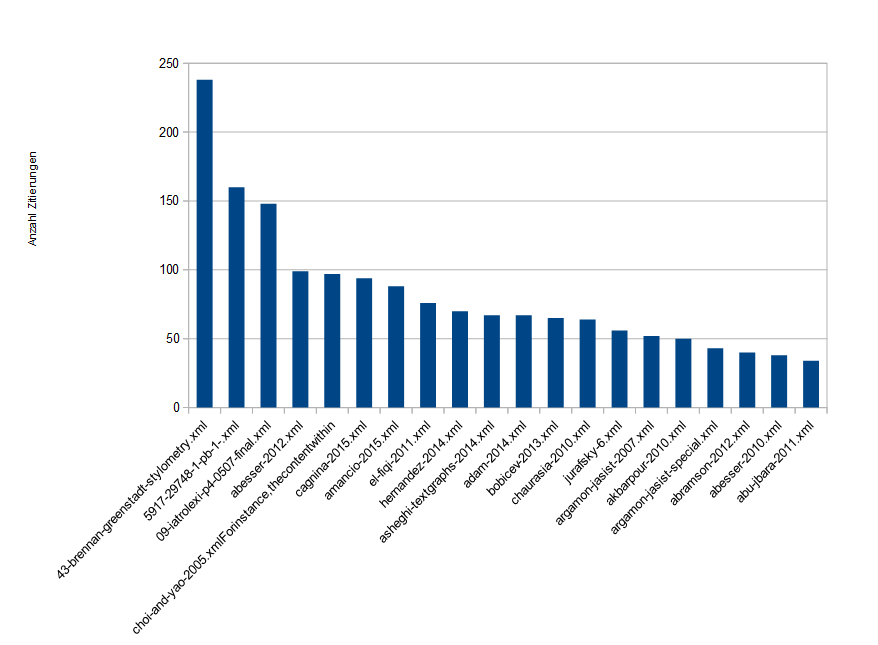
\includegraphics[width=\linewidth]{anzahl_zitierungen}
  \caption[]{Anzahl der Zitierungen für die top 20 Paper}
\label{fig:paperrank}
\end{figure}



Zum Abschluss wurden die entsprechenden gezählten Zitierungen in die Ausgangsdateien geschrieben. Sie wurden in <entry>- und <counter>-Tags verpackt, damit im Scoring Schritt ein reibungsloser Zugriff möglich wird.
Nun soll noch ein kurzer Ausblick gegeben werden, was nicht in das Resultat des Paperranks eingeflossen ist, aber die Ergebnisse noch verbessern könnte. Bei der Extraktion der Quellen ist sicher noch einiges an Optimierungspotenzial. Es könnten weitere Kriterien in die Auswahl einfließen, um zum einen mehr Quellen zu finden und zum anderen \emph{Nichtquellen} zu eliminieren. Außerdem wurde nicht beachtet, welche Quelle die Zitierungen vornimmt. Generell hat sich das Vorgehen an keinem Algorithmus, wie bspw. dem Random Surfer Modell orientiert. Dies wäre auch ein interessanter Ansatz für weitere Nachforschungen. 
Nichtsdestotrotz entstand mit dieser Arbeit eine weitere Möglichkeit die gegebenen wissenschaftlichen Texte zu bewerten bzw. zu \emph{ranken}. Des Weiteren ist nun eine Aussage darüber möglich, wie oft einzelne Paper in anderen Papern als Quellen herangezogen werden und wie die  Verteilung über alle Texte ist.



%%% Local Variables:
%%% mode: latex
%%% TeX-master: "../arbeit"
%%% End:


\chapter{Indexierung}\label{ch:indexing}
Die aus der Vorverarbeitung erstellten XML-Dokumente werden mit
\lucene \lstinline{7.1.0} indiziert.  Da einzelne Abschnitte
bzw. Elemente des XML-Dokuments abgreifbar sind, können sie in
einzelne Felder des Lucene-Dokuments gespeichert werden.  Zu den
Feldern, die aufgenommen wurden gehören Titel, Autor,
Publikationsdatum und der Content als Fließtext einer Publikation,
sowie Dateiname und -pfad des PDF-Dokuments, und die ID des
XML-Dokuments.  Des Weiteren wurde die Anzahl, wie oft eine
Publikation von den anderen Publikationen in der PDF-Kollektion
zitiert wurde, in ein Feld aufgenommen, um diesen Wert später beim
Scoring nutzen zu können.  Für die Indizierung wird die Klasse
\lstinline{de.uni_leipzig.digital_text_forensics.lucene.Main}
aufgerufen, welche wiederum die Klassen
\lstinline{de.uni_leipzig.digital_text_forensics.lucene.XMLFileIndexer}
aufruft, die als Konstruktor den Pfad zum Lucene-Index erhält.

Die Suche ist in der Klasse \lstinline{de.uni_leipzig.digital_text_forensics.lucene.Searcher} implementiert. 
Um sowohl im Titel-Feld des Dokuments, als auch im Content-Feld suchen zu können, wurde das \lstinline{MultiFieldQueryParser}-Objekt von \lucene genutzt. 
Um Suchanfragen, die zu Beginn des Dokuments vorkommen, höher zu gewichten, wurde das \lstinline{SpanFirstQuery}-Objekt genutzt. 
Weiterhin werden Wörter, die im Titel-Feld des Dokuments stärker gewichtet als Wörter, die im Content-Feld des Dokuments vorkommen. 
Dazu wird dem Konstruktor des \lstinline{MultiFieldQueryParser}-Objekts eine \lstinline{HashMap} mit Key-Value-Paaren übergeben. 
Key ist das Feld (z.\,B. Titel), Value ist der Faktor mit dem das Feld gewichtet wird. 
Für das Titel-Feld wurde der Wert $0.8$ gewählt, für das Content-Feld $0.2$. 
Dies ist damit zu begründen, dass das Vorkommen der Suchanfrage, oder Teile davon, im Titel eines Dokuments ein Indikator für eine höhere Relevanz des Dokuments ist.  
Das Scoring für die Relevanz eines Dokuments für eine Suchanfrage setzt sich nun folgendermaßen zusammen: 
\begin{itemize} 
	\item Aus dem von \lucene intern berechneten Gewichtswert für die Relevanz eines Dokuments. 
	\item Aus der Anzahl, wie oft eine Publikation zitiert wurde. 
	\item Aus der Anzahl der Clicks, ein Dokument für eine Suchanfrage erhalten hat. 
	\item Aus der Zeitspanne, die Nutzer im Durchschnitt auf einem Dokument verbracht haben. 
\end{itemize}
Die letzten drei Faktoren der Liste werden dem von \lucene berechneten Gewichtswert aufaddiert. 
Werte für Clickzahl und Zeitspanne werden dabei aus dem Backend zur Verfügung gestellt. 
Die Anzahl, wie oft eine Publikation zitiert wurde, wird in der Vorverarbeitung direkt im XML-Dokument gespeichert und ist dadurch abgreifbar. 
Da die einzelnen Gewichtsfaktoren unterschiedliche Größenordnungen annehmen können, mussten sie normiert werden. 
Dazu wurde der Tangens hyperbolicus herangezogen, um Werte zwischen $0$ und $1$ zu erhalten. 
Dann wurde ein Gewichtswert festgelegt und aufmultipliziert. 

Für die Präsentation der Suchergebnisse werden Snippets generiert, die das Vorkommen der Suchanfrage in dem Dokument durch Highlighting der entsprechenden Wörter kenntlich macht. Dabei wurde die Länge eines Snippets auf $400$ Zeichen festgelegt. 
%%% Local Variables:
%%% mode: latex
%%% TeX-master: "../arbeit"
%%% End:


\chapter{Backend}\label{ch:backend}

%%% Local Variables:
%%% mode: latex
%%% TeX-master: "../arbeit"
%%% End:

\section{Auswahl eines Backend-Frameworks}
Zuerst wurde für die Programmierung einer Webanwendung ein geeignetes Framework gesucht, um Programmier-Paradigmen umzusetzen und die Architektur besser zu abstrahieren. 
Hierfür wurden zahlreiche Frameworks untersucht, welche Dependency Injection (DI), Inversion of Control (IoC) und Aspect-Oriented Programming (AOP) unterstützen.
Aufgrund der Auswahl der Programmiersprache Java für die Umsetzung der Anwendung schränkte sich die Anzahl der Frameworks ein.
Die Recherche ergab folgende drei Frameworks:

\begin{table}[h!]
	\centering
	
	\begin{tabularx}{\textwidth}{|l|c|X|}
		
		\hline
		\multicolumn{1}{|c|}{{\textbf{Frameworks}}} & \multicolumn{1}{c|}{{\textbf{Sprache}}} & \multicolumn{1}{c|}{{\textbf{Eigenschaft}}} \\
		\hline	     
		
		HiveMid & Java & DI, AOP-ähnliches Feature, IoC Container \\
		
		Google Guice & Java & DI, AOP, IoC Container,  Annotations, Generics, modular\\
		
		Spring Boot & Java & DI, AOP, IoC Container,  Annotations, Generics, modular\\
		\hline
	\end{tabularx}
	\caption{DI-Frameworks}
	\label{tbl:diFrameworks}
\end{table}

HiveMind und Google Guice bieten gegenüber Spring Boot leichter verständliche Programmierungstechniken sowie einen prägnanteren und lesbareren Code.
HiveMind fokussiert sich auf das Verbinden von Services. 
Seine Konfiguration erfolgt über eine XML-Datei oder eine eigene Definitions-Sprache. 
Hierdurch ist HiveMind ein kleiner und simpel gestalteter DI-Container.
Darüber hinaus  bietet HiveMind die Möglichkeit, mit AOP zu arbeiten.
Google Guice hingegen unterstützt Features wie Annotations und Generics, die ab Java 1.5 zur Verfügung stehen. 
Sie helfen dabei, eine weitgehend aufgeräumte und einfache Konfiguration zu ermöglichen.
Google Guice und Spring Boot bieten sehr ähnliche Ansätze und kommen mit vielen Anforderungen, die Unternehmenssoftware erfüllen müssen, zurecht.
Google Guice ist durch die geringere Komplexität leichter zu verstehen und insgesamt kleiner als Spring Boot.
Jedoch bietet die Modularität von Spring Boot den größeren Vorteil:
Die Module können, je nachdem welche der Entwickler benötigt, ohne viel Aufwand hinzugefügt werden.
Schlussendlich fiel die Entscheidung auf das Spring Boot-Framework, da dessen Flexibilität und Modularität die Entwicklung von Anwendungen stark vereinfacht und daher die beste Wahl darstellt.

\section{Auswahl einer Datenbank}
Als nächstes wurde für das spätere Speichern der Interaktion zwischen Backend, Suchergebnissen und User, genauer des User-Feedbacks eine geeignetes eingebettetes Datenbanksystem gesucht. 
Die Recherche ergab folgende Datenbanken:

\begin{table}[h!]
	\centering
	
	\begin{tabularx}{\textwidth}{|l|c|X|}
		
		\hline
		\multicolumn{1}{|c|}{{\textbf{Datenbank}}} & \multicolumn{1}{c|}{{\textbf{Sprache}}} & \multicolumn{1}{c|}{{\textbf{Eigenschaft}}} \\
		\hline	     
		SQLite & C & SQL-92-Standard,  Transaktionen, Unterabfragen (Subselects), Sichten (Views), Trigger und benutzerdefinierte Funktionen, direkte Integration in Anwendungen, In-Memory-Datenbank \\
		\hline
		Apache Cassandra & Java & Spaltenorientierte NoSQL-Datenbank, für sehr große strukturierte Datenbanken, hohe Skalierbarkeit und Ausfallsicherheit bei großen, verteilten Systemen \\
		\hline
		H2 & Java &   Schnell, Referenzielle Integrität, Transaktionen, Clustering, Datenkompression, Verschlüsselung und SSL, direkte Einbettung in Java-Anwendungen oder Betrieb als Server möglich, direkte Unterstützung in Spring Boot, In-Memory-Datenbank \\
		\hline
		
	\end{tabularx}
	\caption{Datenbanken}
	\label{tbl:dbs}
\end{table}

SQLite bietet einen leichten Einstieg in die Datenbanken.
Dabei stellt SQLite den größten Teil des SQL-92-Standards zur Verfügung und kann Transaktionen, Unterabfragen und viele weitere Funktionen durchführen.
Außerdem ist es eine In-Memory-Datenbank. 
Jedoch unterstützt Spring Boot diese Datenbank nicht von Haus aus und es müssten aufwendige Konfiguration vorgenommen werden.

Apache Cassandra ist eine spaltenorientierte NoSQL-Datenbank und ist für große strukturierte Daten, hohe Skalierbarkeit und Ausfallsicherheit ausgelegt.
Für das vorliegende Projekt ist Apache Cassandra jedoch zu groß ausgelegt, da für das Backend mit geringeren Datenmengen gearbeitet werden soll.

H2 ist eine In-Memory-Datenbank, welche schnell ist und referenzielle Integrität, Transaktionen, Clustering sowie  Datenkompression unterstützt.
Außerdem kann Spring Boot mit dieser Datenbank ohne besondere Maßnahmen wie aufwändige Konfigurationen verwendet und in die vorliegende Anwendung integriert werden.
Deshalb wurde entschlossen, H2 als Datenbank anzuwenden.

\section{Erstellung des Backends}
Nach der Auswahl der Backendtechnologien wurde die Grundarchitektur des Backends konzipiert und implementiert.

\subsection{Kommunikation mit der Datenbank}
Zunächst wurden Datenmodels wie \texttt{Query} oder \texttt{LoggingDocument} erstellt. 
Hieraus werden später die Tabellen der Datenbank generiert.
Um mit der Datenbank kommunizieren zu können, werden Data Access Objects (DAO) als Kommunikationsschnittstellen erstellt. 
Ein DAO hat eine Anbindung zu den Spring-Boot Repositorys, welche in der Lage sind SQL-Query zu generieren und übermittelt diese an die Datenbank.
Beispiele hierfür sind das Speichern und Abrufen von \texttt{LoggingDocument}-Daten, welche einen Teil des User-Feedbacks darstellen.
\begin{lstlisting}
public interface LoggingDocDao extends JpaRepository<LoggingDocument, Long> {
LoggingDocument findByDocId(Long docId);
}
\end{lstlisting}

Im obigen Code-Ausschnitt wird mit Hilfe von Spring Boot die SQL-Qyery \texttt{findByDocId} aus dem \texttt{LoggingDocument} generiert.
Dies findet über den Namen eines Interfaces statt.
Die einzelnen Komponenten, welche implementiert wurden, kommunizieren nicht direkt über die DAOs mit der Datenbank, sondern über ein Interface.
Dadurch ist eine lose Kopplung zwischen den Komponenten, DAOs und der Datenbank möglich.
Damit ist die Datenbank ohne große Änderungen in den Implementierungen austauschbar. 
Folglich fehlen nur noch Änderungen in den Konfigurationen und eventuell in den DAOs.
 
\begin{lstlisting}
public class LoggingDocServiceImpl implements LoggingDocService {
	public LoggingDocument findbyId(Long id) {
	return loggingDocDao.findOne(id);
	}}
\end{lstlisting}
Im vorliegenden Listing ist \texttt{LoggingDocService} als Beispiel für einen Service dargestellt.
In der Implantation des Interfaces wird nun das DAO aufgerufen, beispielsweise die Methode \texttt{findbyId}.

\subsection{Controller}
Im nächsten Schritt wurden sogenannte Controller erstellt.
Diese bilden eine wichtige Schnittstelle für die Kommunikation mit dem Frontend und Backend.
Controller reagieren auf HTTP-Requests, welche von dem Frontend oder anderen Clients gesendet werden.
Die Aufgabe ist es, für bestimmte Ressource-URLs spezielle Ereignisse auszuführen.
Ein Beispiel hierfür ist Auswertung der Suchanfrage der Search-Zeile im Frontend  und das Rücksenden der Suchergebnisse.
\begin{lstlisting}
@RequestMapping(method = RequestMethod.GET, path = "/")
public ModelAndView searchPage(
@RequestParam(defaultValue = "")
String query) {
ModelAndView modelAndView = new ModelAndView("search");
...
List<ScoreDoc> list = querySearcher.search(query);
...
modelAndView.addObject("searchResultPage", searchResultPage);
return modelAndView;}
\end{lstlisting}

Im obigen Code-Beispielabschnitt ist erkennbar, dass, beim Auslösen eines Request bei der Path-URL \texttt{\glqq/\grqq~} die Funktion \texttt{SearchPage} aufgerufen und eine Suche ausgeführt wird.
Hierfür wird der Request-Parameter mit \texttt{query} ausgewertet.
Die Suche erfolgt mithilfe der Komponente Lucene, welche bereits in Abschnitt \ref{ch:indexing} näher erläutert wurde.
Im Anschluss werden die Suchergebnisse als \texttt{modelAndView}-Objekt dem Frontend übergeben. 

\subsection{Komponenten des Frontends}
Nach dem Controller wurden die Komponenten, welche für das Frontend benötigt werden, konzipiert und im Anschluss implementiert. 

Wurden die Suchen durchgeführt und die Lucene-Komponente die Suchergebnisse zurückgegeben, wird die gesamte Ergebnisliste gesplittet.
Hierbei wird für die angeforderte Seite eine Subliste erstellt, in welcher nur die geforderten Suchergebnisse enthalten sind und die restlichen Ergebnisse verworfen werden.
Hierdurch ist es nicht erforderlich, alle Ergebnisse zu transformieren.
Dadurch arbeitet die Anwendung wesentlich schneller.

Als nächstes wurde ein Data Transfer Object (DTO) erstellt, um die relevanten Suchergebnisse, die in der Subliste enthalten sind, in das gewünschte Ausgabeformat zu überführen und in einer separaten  Liste zu sammeln.
Das DTO hat dabei unter anderem die Variablen Autor, Titel, Snippet oder den Redirect-Link, welcher auf die zugehörige PDF zeigt.   
Der Link hierfür wird mit der Methode \texttt{createLink} erzeugt.
Zu diesem Zweck werden aus der docId, Query und dem Host ein Link erstellt. 
Als Beispiel wird folgender Link generiert:

\textit{http://localhost:8080/pdf/?docId=1\&query=xyz}.

Der Parameter \texttt{docId} ist dabei eine Id, welche die PDF zu dem Suchergebnis angibt und der Parameter \texttt{query} dient dem User-Feedback.
Beim späteren Klick auf das Suchergebnis wird zum einen die dazugehörige PDF angezeigt und zum anderen gleichzeitig in der Datenbank das Dokument, welches mit dem einer bestimmten Query gefunden wurde, gespeichert.
Damit ist es möglich, Rückschlüsse auf die Wichtigkeit des Dokuments zu ziehen.
Der eben beschriebene Vorgang erfolgt mit der Methode \texttt{mapDocumentListToSearchResults}.
Nach dem Erstellen der Liste der transformierten Suchergebnisse, wird sie zum Objekt \texttt{searchResultPage} hinzugefügt und um weitere Angaben ergänzt.
Das ist im folgenden Code-Abschnitt ausschnittsweise zu sehen.
\pagebreak

\begin{lstlisting}
List<ScoreDoc> split = pager.split(list, currentPage);
searchResultList = querySearcher.mapDocumentListToSearchResults(split,query);
searchResultPage.setTotalResults(list.size());
searchResultPage.setResultsOnPage(searchResultList);
searchResultPage.setPage(currentPage);
\end{lstlisting}

Hinzu zum Beispiel kommt die Gesamtanzahl an Suchergebnissen oder auf welcher Page man sich befindet.

Die \texttt{searchResultPage} wird nun der Spring Boot Thymeleaf-Komponente übergeben und die \texttt{search.html}-Page erstellt.
Hierfür wurde ein \texttt{search.html}-Template erstellt, in welchem Anweisungen zum Umgang mit den übergebenden Daten gegeben werden.
Thymeleaf befolgt diese Anweisungen und wandelt sie in entsprechende HTML-Komponenten um, damit im Anschluss der der Umwandlung ein Webbrowser die Page anzeigen kann.
Ein Beispiel der Anweisungen für Thymeleaf wird im folgenden Code-Abschnitt aufgezeigt.

\begin{lstlisting}
<div th:each="result : ${searchResultPage.resultsOnPage}">
	<h3 class="card-title">
		<a th:href="${result.webUrl.href}"
			th:text="${result.title}">
		</a>
	</h3>
</div>
\end{lstlisting}

Das \texttt{searchResultPage}-Objekt wird aufgerufen.
Daraufhin wird in einer Schleife die Liste der DTO-Objekte, die im \texttt{searchResultPage}-Objekt enthalten sind, mit Titel und \texttt{webURL} als HTML h3-Tag, welche einen Link darstellt, erstellt.
Durch die Schleife wird somit für jedes Element ein eigenes HTML-Element generiert.
Die Gestaltung der Oberfläche und deren Elemente wurde in separaten CSS- und Javascript-Dateien vorgenommen.
Nach der Erstellung der \texttt{search.html}-Page wird die fertige Page über den Request zurückgegeben und der Webbrowser zeigt sie an.

\chapter{Frontend}\label{ch:frontend}

Nach dem Controller wurden die Komponenten, welche für das Frontend benötigt werden, konzipiert und im Anschluss implementiert. 

Wurden die Suchen durchgeführt und die Lucene-Komponente die Suchergebnisse zurückgegeben, wird die gesamte Ergebnisliste gesplittet.
Hierbei wird für die angeforderte Seite eine Subliste erstellt, in welcher nur die geforderten Suchergebnisse enthalten sind und die restlichen Ergebnisse verworfen werden.
Hierdurch ist es nicht erforderlich, alle Ergebnisse zu transformieren.
Dadurch arbeitet die Anwendung wesentlich schneller.

Als nächstes wurde ein Data Transfer Object (DTO) erstellt, um die relevanten Suchergebnisse, die in der Subliste enthalten sind, in das gewünschte Ausgabeformat zu überführen und in einer separaten  Liste zu sammeln.
Das DTO hat dabei unter anderem die Variablen Autor, Titel, Snippet oder den Redirect-Link, welcher auf die zugehörige PDF zeigt.   
Der Link hierfür wird mit der Methode \texttt{createLink} erzeugt.
Zu diesem Zweck werden aus der docId, Query und dem Host ein Link erstellt. 
Als Beispiel wird folgender Link generiert:

\url{http://localhost:8080/pdf/?docId=1\&query=xyz}.

Der Parameter \texttt{docId} ist dabei eine Id, welche die PDF zu dem Suchergebnis angibt und der Parameter \texttt{query} dient dem User-Feedback.
Beim späteren Klick auf das Suchergebnis wird zum einen die dazugehörige PDF angezeigt und zum anderen gleichzeitig in der Datenbank das Dokument, welches mit dem einer bestimmten Query gefunden wurde, gespeichert.
Damit ist es möglich, Rückschlüsse auf die Wichtigkeit des Dokuments zu ziehen.
Der eben beschriebene Vorgang erfolgt mit der Methode \texttt{mapDocumentListToSearchResults}.
Nach dem Erstellen der Liste der transformierten Suchergebnisse, wird sie zum Objekt \texttt{searchResultPage} hinzugefügt und um weitere Angaben ergänzt.
Das ist im folgenden Code-Abschnitt ausschnittsweise zu sehen.
\pagebreak

\begin{lstlisting}
List<ScoreDoc> split = pager.split(list, currentPage);
searchResultList = querySearcher.mapDocumentListToSearchResults(split,query);
searchResultPage.setTotalResults(list.size());
searchResultPage.setResultsOnPage(searchResultList);
searchResultPage.setPage(currentPage);
\end{lstlisting}

Hinzu zum Beispiel kommt die Gesamtanzahl an Suchergebnissen oder auf welcher Page man sich befindet.

Die \texttt{searchResultPage} wird nun der Spring Boot Thymeleaf-Komponente übergeben und die \texttt{search.html}-Page erstellt.
Hierfür wurde ein \texttt{search.html}-Template erstellt, in welchem Anweisungen zum Umgang mit den übergebenden Daten gegeben werden.
Thymeleaf befolgt diese Anweisungen und wandelt sie in entsprechende HTML-Komponenten um, damit im Anschluss der der Umwandlung ein Webbrowser die Page anzeigen kann.
Ein Beispiel der Anweisungen für Thymeleaf wird im folgenden Code-Abschnitt aufgezeigt.

\begin{lstlisting}
<div th:each="result : ${searchResultPage.resultsOnPage}">
	<h3 class="card-title">
		<a th:href="${result.webUrl.href}"
			th:text="${result.title}">
		</a>
	</h3>
</div>
\end{lstlisting}

Das \texttt{searchResultPage}-Objekt wird aufgerufen.
Daraufhin wird in einer Schleife die Liste der DTO-Objekte, die im \texttt{searchResultPage}-Objekt enthalten sind, mit Titel und \texttt{webURL} als HTML h3-Tag, welche einen Link darstellt, erstellt.
Durch die Schleife wird somit für jedes Element ein eigenes HTML-Element generiert.
Die Gestaltung der Oberfläche und deren Elemente wurde in separaten CSS- und Javascript-Dateien vorgenommen.
Nach der Erstellung der \texttt{search.html}-Page wird die fertige Page über den Request zurückgegeben und der Webbrowser zeigt sie an.

\chapter{Evaluation und Fazit}\label{ch:results}

%%% Local Variables:
%%% mode: latex
%%% TeX-master: "../arbeit"
%%% End:






%%% könnt ihr gerne benutzen, seh hier aber keinen Mehrwert.

% Literaturverzeichnis
%\bibliography{bibliography}
% \printbibliography[heading=bibintoc]

\newpage
\appendix

\chapter{Abbildungen, Tabellen und Listings}\label{ch:results}

\begin{figure}[ht]

    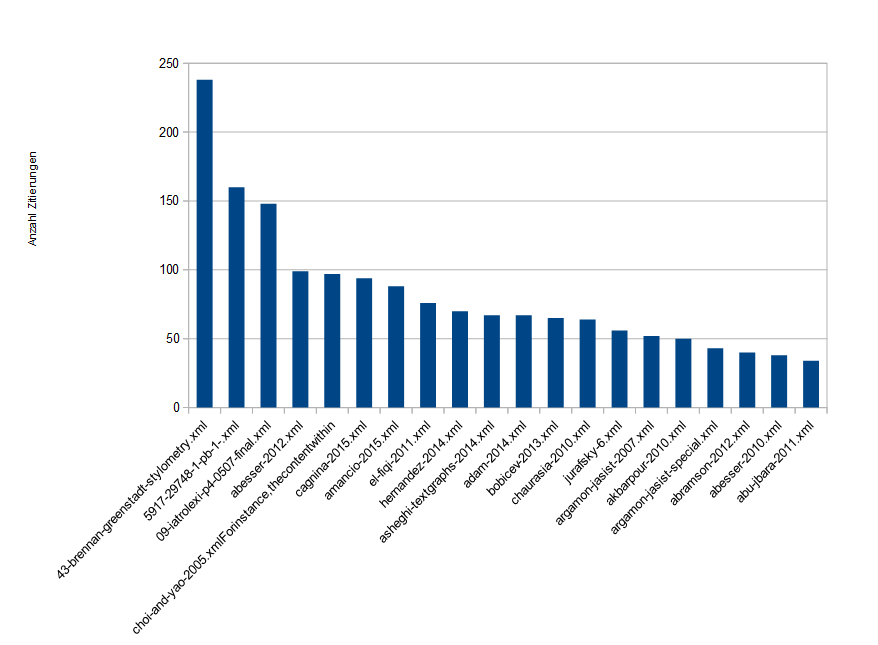
\includegraphics[width=\linewidth]{anzahl_zitierungen}
  \caption[]{Anzahl der Zitierungen für die top 20 Paper}
\label{fig:paperrank}
\end{figure}


\end{document}

%%% Local Variables:
%%% mode: latex
%%% TeX-master: t
%%% End:
